% *********************************************************************
% © 2016–2026 Jeremy Sylvestre
%
% Permission is granted to copy, distribute and/or modify this document
% under the terms of the GNU Free Documentation License, Version 1.3 or
% any later version published by the Free Software Foundation; with no
% Invariant Sections, no Front-Cover Texts, and no Back-Cover Texts. A
% copy of the license is included in the appendix entitled “GNU Free
% Documentation License” that appears in the output document of this
% PreTeXt source code. All trademarks™ are the registered® marks of
% their respective owners.
%
% *********************************************************************
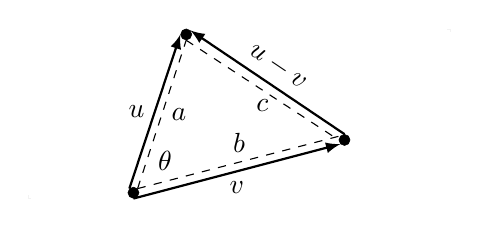
\begin{tikzpicture}[
	point/.style={circle,draw,very thin,fill,inner sep=0pt,minimum size=4pt},
	vector/.style={-latex},
	scale=0.67
]
	% artificially widen image to widen room for its caption
	% as it is part of a sidebyside
	% actual dimensions are ~ (0,0) to (4,3)
	\draw[black!5!white,very thin] (-2,-0.05) to (-2,-0.1) to (-1.95,-0.1);
	\draw[black!5!white,very thin] (5.95,3.1) to (6,3.1) to (6,3.05);

	\node[point] at (0,0) (o) {};
	\node[point] at (1,3) (u) {};
	\node[point] at (4,1) (v) {};
	\draw[vector,thick] (o.north west) to node[left] {$\uvec{u}$} (u.west);
	\draw[dashed] (o.north east) to node[right] {$a$} (u.south);
	\draw[vector,thick] (o.south) to node[below] {$\uvec{v}$} (v.south west);
	\draw[dashed] (o.north east) to node[above] {$b$} (v.north west);
	\draw[vector,thick] (v.north) to node[above,sloped] {$\uvec{u} - \uvec{v}$} (u.north east);
	\draw[dashed] (u.south) to node[below] {$c$} (v.west);
	\node at (0.6,0.6) {$\theta$};
\end{tikzpicture}
